% Options for packages loaded elsewhere
% Options for packages loaded elsewhere
\PassOptionsToPackage{unicode}{hyperref}
\PassOptionsToPackage{hyphens}{url}
\PassOptionsToPackage{dvipsnames,svgnames,x11names}{xcolor}
%
\documentclass[
  letterpaper,
  DIV=11,
  numbers=noendperiod]{scrartcl}
\usepackage{xcolor}
\usepackage{amsmath,amssymb}
\setcounter{secnumdepth}{-\maxdimen} % remove section numbering
\usepackage{iftex}
\ifPDFTeX
  \usepackage[T1]{fontenc}
  \usepackage[utf8]{inputenc}
  \usepackage{textcomp} % provide euro and other symbols
\else % if luatex or xetex
  \usepackage{unicode-math} % this also loads fontspec
  \defaultfontfeatures{Scale=MatchLowercase}
  \defaultfontfeatures[\rmfamily]{Ligatures=TeX,Scale=1}
\fi
\usepackage{lmodern}
\ifPDFTeX\else
  % xetex/luatex font selection
\fi
% Use upquote if available, for straight quotes in verbatim environments
\IfFileExists{upquote.sty}{\usepackage{upquote}}{}
\IfFileExists{microtype.sty}{% use microtype if available
  \usepackage[]{microtype}
  \UseMicrotypeSet[protrusion]{basicmath} % disable protrusion for tt fonts
}{}
\makeatletter
\@ifundefined{KOMAClassName}{% if non-KOMA class
  \IfFileExists{parskip.sty}{%
    \usepackage{parskip}
  }{% else
    \setlength{\parindent}{0pt}
    \setlength{\parskip}{6pt plus 2pt minus 1pt}}
}{% if KOMA class
  \KOMAoptions{parskip=half}}
\makeatother
% Make \paragraph and \subparagraph free-standing
\makeatletter
\ifx\paragraph\undefined\else
  \let\oldparagraph\paragraph
  \renewcommand{\paragraph}{
    \@ifstar
      \xxxParagraphStar
      \xxxParagraphNoStar
  }
  \newcommand{\xxxParagraphStar}[1]{\oldparagraph*{#1}\mbox{}}
  \newcommand{\xxxParagraphNoStar}[1]{\oldparagraph{#1}\mbox{}}
\fi
\ifx\subparagraph\undefined\else
  \let\oldsubparagraph\subparagraph
  \renewcommand{\subparagraph}{
    \@ifstar
      \xxxSubParagraphStar
      \xxxSubParagraphNoStar
  }
  \newcommand{\xxxSubParagraphStar}[1]{\oldsubparagraph*{#1}\mbox{}}
  \newcommand{\xxxSubParagraphNoStar}[1]{\oldsubparagraph{#1}\mbox{}}
\fi
\makeatother


\usepackage{longtable,booktabs,array}
\usepackage{calc} % for calculating minipage widths
% Correct order of tables after \paragraph or \subparagraph
\usepackage{etoolbox}
\makeatletter
\patchcmd\longtable{\par}{\if@noskipsec\mbox{}\fi\par}{}{}
\makeatother
% Allow footnotes in longtable head/foot
\IfFileExists{footnotehyper.sty}{\usepackage{footnotehyper}}{\usepackage{footnote}}
\makesavenoteenv{longtable}
\usepackage{graphicx}
\makeatletter
\newsavebox\pandoc@box
\newcommand*\pandocbounded[1]{% scales image to fit in text height/width
  \sbox\pandoc@box{#1}%
  \Gscale@div\@tempa{\textheight}{\dimexpr\ht\pandoc@box+\dp\pandoc@box\relax}%
  \Gscale@div\@tempb{\linewidth}{\wd\pandoc@box}%
  \ifdim\@tempb\p@<\@tempa\p@\let\@tempa\@tempb\fi% select the smaller of both
  \ifdim\@tempa\p@<\p@\scalebox{\@tempa}{\usebox\pandoc@box}%
  \else\usebox{\pandoc@box}%
  \fi%
}
% Set default figure placement to htbp
\def\fps@figure{htbp}
\makeatother





\setlength{\emergencystretch}{3em} % prevent overfull lines

\providecommand{\tightlist}{%
  \setlength{\itemsep}{0pt}\setlength{\parskip}{0pt}}



 


\KOMAoption{captions}{tableheading}
\makeatletter
\@ifpackageloaded{caption}{}{\usepackage{caption}}
\AtBeginDocument{%
\ifdefined\contentsname
  \renewcommand*\contentsname{Table of contents}
\else
  \newcommand\contentsname{Table of contents}
\fi
\ifdefined\listfigurename
  \renewcommand*\listfigurename{List of Figures}
\else
  \newcommand\listfigurename{List of Figures}
\fi
\ifdefined\listtablename
  \renewcommand*\listtablename{List of Tables}
\else
  \newcommand\listtablename{List of Tables}
\fi
\ifdefined\figurename
  \renewcommand*\figurename{Figure}
\else
  \newcommand\figurename{Figure}
\fi
\ifdefined\tablename
  \renewcommand*\tablename{Table}
\else
  \newcommand\tablename{Table}
\fi
}
\@ifpackageloaded{float}{}{\usepackage{float}}
\floatstyle{ruled}
\@ifundefined{c@chapter}{\newfloat{codelisting}{h}{lop}}{\newfloat{codelisting}{h}{lop}[chapter]}
\floatname{codelisting}{Listing}
\newcommand*\listoflistings{\listof{codelisting}{List of Listings}}
\makeatother
\makeatletter
\makeatother
\makeatletter
\@ifpackageloaded{caption}{}{\usepackage{caption}}
\@ifpackageloaded{subcaption}{}{\usepackage{subcaption}}
\makeatother
\usepackage{bookmark}
\IfFileExists{xurl.sty}{\usepackage{xurl}}{} % add URL line breaks if available
\urlstyle{same}
\hypersetup{
  pdftitle={PRS Analysis for WSL},
  colorlinks=true,
  linkcolor={blue},
  filecolor={Maroon},
  citecolor={Blue},
  urlcolor={Blue},
  pdfcreator={LaTeX via pandoc}}


\title{PRS Analysis for WSL}
\author{Lukas Graz}
\date{2025-02-25}
\begin{document}
\maketitle


For the \textbf{release notes} see the corresponding
\href{https://github.com/LGraz/wsl--prs-analysis/releases}{GitHub} page

\section{Data Preparation}\label{data-preparation}

\subsection{Train Test Split for
Inference}\label{train-test-split-for-inference}

Data was split into training and test sets (50/50) for hypothesis
testing to ensure valid inference after feature selection.

\subsection{Missing Values}\label{missing-values}

Missing value imputation was performed using MissForest
doi:10.1093/bioinformatics/btr597. This method leverages conditional
dependencies between variables to predict missing values through an
iterative random forest approach.

To avoid introducing spurious correlations between different variable
sets, we imputed the following data groups separately:

\begin{itemize}
\tightlist
\item
  PRS variables on the complete dataset
\item
  Mediators on training data only
\item
  GIS variables on training data only
\item
  Mediators for prediction analysis
\item
  GIS variables for prediction analysis
\item
  PRS variables for prediction analysis
\end{itemize}

Mediators and GIS variables were intentionally not imputed on the test
set to maintain valid inference, as MissForest does not provide a
mechanism to propagate imputation uncertainty. An alternative would be
the \texttt{mice}-routine, which could be implemented in future
analyses. Missing values in the test set predictors remained untreated,
which is justified under the missing completely at random (MCAR)
assumption---where missing values occur independently of all other
variables.

For the prediction analysis, fewer statistical assumptions are required,
so using the MissForest approach does not violate any assumptions.

PRS variables could have been imputed separately for training/test sets
and prediction analysis, but we prioritized simplicity as these
variables serve only as response variables.

Additionally, we compared MissForest with simpler imputation methods
(variable-wise and observation-wise mean imputation) for the PRS
variables. Results confirmed that MissForest consistently outperformed
these alternatives.

\section{Main Analysis}\label{main-analysis}

\subsection{Response Variable
Selection}\label{response-variable-selection}

\begin{itemize}
\tightlist
\item
  Aggregated mean
\item
  FA (Fascination)
\item
  BA (Being Away)
\item
  EC (Extent Coherence)
\item
  ES (Compatibility)
\end{itemize}

\textbf{PCA Verification} of this approach. Key findings:

\begin{itemize}
\tightlist
\item
  Data can be well approximated with 3-4 dimensions
\item
  First dimension is close to weighted average of all variables
  (correlation \textgreater0.99)
\item
  EC (Extent Coherence) shows most divergence (see PC2)
\item
  FA (Fascination) and BA (Being Away) show similarity (see PC1-PC3)
\item
  Aggregated PRS variables justified by PCA results (similar rotation
  values), supporting use of mean
\end{itemize}

\subsection{Prediction Analysis with Machine Learning
Methods}\label{prediction-analysis-with-machine-learning-methods}

Details and results in \href{notebooks/mlr3.qmd}{the notebook}.

This section investigates predictive relationships between Perceived
Restorativeness Scale (PRS) variables, mediator variables, and
Geographical Information System (GIS) variables using various machine
learning approaches. We employed a systematic methodology to quantify
the predictive power of different variable combinations.

\subsubsection{Methodological Approach}\label{methodological-approach}

We evaluated multiple machine learning models using the mlr3 framework
(cite doi:10.21105/joss.01903) :

\begin{itemize}
\tightlist
\item
  Linear models (baseline)
\item
  XGBoost (gradient boosting with tree-based models and hyperparameter
  tuning for learning rate and tree depth) (cite arxiv:1603.02754)
\item
  Random Forests (with default parameters) (cite
  doi:10.1023/A:1010933404324)
\end{itemize}

Performance was measured as percentage of explained variance on hold-out
data, calculated as (1 - MSE/Variance(y)), where MSE represents mean
squared error.

\subsubsection{Model Combinations}\label{model-combinations}

To systematically explore predictive relationships, we tested four model
configurations:

\begin{enumerate}
\def\labelenumi{\arabic{enumi}.}
\tightlist
\item
  PRS \textasciitilde{} GIS: Predicting PRS variables using only GIS
  variables
\item
  PRS \textasciitilde{} GIS + Mediators: Predicting PRS variables using
  both GIS and mediator variables
\item
  PRS \textasciitilde{} Mediators: Predicting PRS variables using only
  mediator variables
\item
  Mediators \textasciitilde{} GIS: Predicting mediator variables using
  GIS variables
\end{enumerate}

\subsubsection{Results}\label{results}

\begin{itemize}
\tightlist
\item
  GIS shows limited predictive power for PRS on ES (5\% variance
  explained)
\item
  GIS + Mediators explain 25\% of PRS variance
\item
  Mediators alone explain majority of PRS variance

  \begin{itemize}
  \tightlist
  \item
    GIS primarily helps with ES through tree-based methods
  \item
    Suggests GIS effect is more interaction-based than direct
  \item
    Similar reduction in tree-based methods observed in BA
  \end{itemize}
\end{itemize}

\subsection{Hypothesis Testing: Investigation of Variable Effects on
Perceived Restorativeness
Scale}\label{hypothesis-testing-investigation-of-variable-effects-on-perceived-restorativeness-scale}

Details and results in \href{notebooks/hypothethis-tests.qmd}{the
notebook}.

Here we investigated which variables (including their interactions)
influence PRS variables using multiple linear regression. With 190
variables (counting interactions), the variance inflation factor (VIF)
was high and the multiple testing problem severe. We therefore
implemented a stepwise feature selection using Bayesian Information
Criterion (BIC) on the training data, starting with an empty model to
help computational complexity. Selected features were subsequently used
to fit models on the test set to obtain valid p-values. To keep the
coefficients interpretable in the presence of interactions, each
variable is scaled to mean 0 and standard deviation 1.

\subsubsection{Model Specification and
Analysis}\label{model-specification-and-analysis}

The analysis systematically explored two key relationship pathways:

\begin{enumerate}
\def\labelenumi{\arabic{enumi}.}
\tightlist
\item
  Mediators \textasciitilde{} (GIS)² - examining how environmental
  features predict psychological mediators
\item
  PRS \textasciitilde{} (Mediators + GIS)² - investigating how both
  environmental features and psychological mediators contribute to
  perceived restorativeness
\end{enumerate}

For each target variable, we constructed a separate model using stepwise
selection and evaluated it on the test dataset.

\subsubsection{Results}\label{results-1}

\begin{itemize}
\tightlist
\item
  For HM\_Noise (now removed): Continuous mediator outperforms
  categorical (scaled to mean 0, sd 1)
\item
  Full \texttt{mice} NA-handling likely unnecessary

  \begin{itemize}
  \tightlist
  \item
    Models use few variables
  \item
    Only LNOISE shows high NA count
  \item
    Information detection still fails
  \end{itemize}
\item
  Significant edges remain in SEM (see all interactions)
\end{itemize}

\paragraph{All Interactions: Mediators \textasciitilde{}
(GIS)\^{}2}\label{all-interactions-mediators-gis2}

Significant codes as usual:
\texttt{0\ \textquotesingle{}***\textquotesingle{}\ 0.001\ \textquotesingle{}**\textquotesingle{}\ 0.01\ \textquotesingle{}*\textquotesingle{}\ 0.05\ \textquotesingle{}.\textquotesingle{}\ 0.1\ \textquotesingle{}\ \textquotesingle{}\ 1}

\begin{longtable}[]{@{}
  >{\raggedright\arraybackslash}p{(\linewidth - 16\tabcolsep) * \real{0.2019}}
  >{\centering\arraybackslash}p{(\linewidth - 16\tabcolsep) * \real{0.0962}}
  >{\centering\arraybackslash}p{(\linewidth - 16\tabcolsep) * \real{0.1058}}
  >{\centering\arraybackslash}p{(\linewidth - 16\tabcolsep) * \real{0.0962}}
  >{\centering\arraybackslash}p{(\linewidth - 16\tabcolsep) * \real{0.1058}}
  >{\centering\arraybackslash}p{(\linewidth - 16\tabcolsep) * \real{0.0962}}
  >{\centering\arraybackslash}p{(\linewidth - 16\tabcolsep) * \real{0.0962}}
  >{\centering\arraybackslash}p{(\linewidth - 16\tabcolsep) * \real{0.0962}}
  >{\centering\arraybackslash}p{(\linewidth - 16\tabcolsep) * \real{0.1058}}@{}}
\toprule\noalign{}
\begin{minipage}[b]{\linewidth}\raggedright
Covariate
\end{minipage} & \begin{minipage}[b]{\linewidth}\centering
FEELNAT
\end{minipage} & \begin{minipage}[b]{\linewidth}\centering
LNOISE
\end{minipage} & \begin{minipage}[b]{\linewidth}\centering
LOC\_SENS
\end{minipage} & \begin{minipage}[b]{\linewidth}\centering
LOC\_SOUN
\end{minipage} & \begin{minipage}[b]{\linewidth}\centering
LOC\_SCEN
\end{minipage} & \begin{minipage}[b]{\linewidth}\centering
LOC\_VISE
\end{minipage} & \begin{minipage}[b]{\linewidth}\centering
LOC\_VEGE
\end{minipage} & \begin{minipage}[b]{\linewidth}\centering
LOC\_FAUN
\end{minipage} \\
\midrule\noalign{}
\endhead
\bottomrule\noalign{}
\endlastfoot
(Intercept) & 0.062 & -0.001 & -0.000 & 0.000 & -0.001 & -0.000 & -0.019
& -0.001 \\
HETER & & & 0.130*** & 0.109** & & & & \\
JNYTIME\_sqrt & & & & & & & -0.114** & \\
LCARTIF\_sqrt & -0.152** & -0.124* & & -0.175*** & & -0.071. & &
-0.214*** \\
LCARTIF\_sqrt:RL\_NDVI & 0.115** & & & & & & & \\
OVDIST\_sqrt & 0.027 & & & & & & & \\
RL\_NDVI & 0.150*** & & & & 0.217*** & & 0.219*** & \\
RL\_NOISE & & -0.242*** & & & & & & \\
STRIMP999\_sqrt & & & -0.073. & & & & & \\
\end{longtable}

\textsubscript{Source:
\href{https://LGraz.github.io/wsl--prs-analysis/index.qmd.html}{Article
Notebook}}

\paragraph{PRS \textasciitilde{} (Mediators +
GIS)\^{}2}\label{prs-mediators-gis2}

Significant codes as usual:
\texttt{0\ \textquotesingle{}***\textquotesingle{}\ 0.001\ \textquotesingle{}**\textquotesingle{}\ 0.01\ \textquotesingle{}*\textquotesingle{}\ 0.05\ \textquotesingle{}.\textquotesingle{}\ 0.1\ \textquotesingle{}\ \textquotesingle{}\ 1}

\begin{longtable}[]{@{}
  >{\raggedright\arraybackslash}p{(\linewidth - 10\tabcolsep) * \real{0.2500}}
  >{\centering\arraybackslash}p{(\linewidth - 10\tabcolsep) * \real{0.1471}}
  >{\centering\arraybackslash}p{(\linewidth - 10\tabcolsep) * \real{0.1618}}
  >{\centering\arraybackslash}p{(\linewidth - 10\tabcolsep) * \real{0.1471}}
  >{\centering\arraybackslash}p{(\linewidth - 10\tabcolsep) * \real{0.1471}}
  >{\centering\arraybackslash}p{(\linewidth - 10\tabcolsep) * \real{0.1471}}@{}}
\toprule\noalign{}
\begin{minipage}[b]{\linewidth}\raggedright
Covariate
\end{minipage} & \begin{minipage}[b]{\linewidth}\centering
MEAN
\end{minipage} & \begin{minipage}[b]{\linewidth}\centering
FA
\end{minipage} & \begin{minipage}[b]{\linewidth}\centering
BA
\end{minipage} & \begin{minipage}[b]{\linewidth}\centering
EC
\end{minipage} & \begin{minipage}[b]{\linewidth}\centering
ES
\end{minipage} \\
\midrule\noalign{}
\endhead
\bottomrule\noalign{}
\endlastfoot
(Intercept) & -0.008 & -0.003 & -0.008 & -0.009 & 0.031 \\
DISTKM\_sqrt & & & & & 0.081* \\
FEELNAT & 0.202*** & 0.169*** & 0.188*** & & 0.258*** \\
FEELNAT:LOC\_SCEN & & -0.002 & & & \\
FEELNAT:LOC\_SENS & 0.054. & & & & \\
LCFOREST\_sqrt & & & & -0.090* & \\
LNOISE & 0.177*** & 0.133*** & & & 0.133** \\
LNOISE:FEELNAT & & & & & -0.006 \\
LOC\_FAUN & & 0.176*** & & & \\
LOC\_SCEN & & 0.164*** & & 0.004 & \\
LOC\_SENS & 0.104* & & 0.147*** & 0.142*** & 0.096* \\
LOC\_VISE & 0.173*** & 0.128** & 0.122** & & \\
RL\_NDVI & & -0.133*** & & & \\
RL\_NDVI:LOC\_SCEN & & 0.024 & & & \\
\end{longtable}

\textsubscript{Source:
\href{https://LGraz.github.io/wsl--prs-analysis/index.qmd.html}{Article
Notebook}}

\subsection{Predict RL via HM}\label{predict-rl-via-hm}

Details/Code and results in \href{notebooks/RL-via-HM.qmd}{the
notebook}.

\textbf{Procedure:} Stepwise feature selection using BIC on training
data and subsequent model fitting on test data. Performed seperately for
\texttt{RL\_NDVI} and \texttt{RL\_NOISE}.

\textbf{Predictors:}:
\texttt{HM\_NDVI\ +\ HM\_NOISE\ +\ LANG\ +\ AGE\ +\ SEX\ +\ SPEED\_log\ +\ JNYTIME\_sqrt}
with all two-way interactions.

\subsubsection{RL\_NDVI}\label{rl_ndvi}

\begin{verbatim}

Call:
lm(formula = formula(step_ndvi), data = D_tst)

Residuals:
   Min     1Q Median     3Q    Max 
-3.371 -0.430  0.182  0.698  1.989 

Coefficients:
                  Estimate Std. Error t value Pr(>|t|)    
(Intercept)        -0.1690     0.0946   -1.79  0.07452 .  
HM_NDVI             0.1581     0.0413    3.83  0.00015 ***
LANGGerman          0.2232     0.1064    2.10  0.03633 *  
LANGItalian         0.0028     0.1965    0.01  0.98866    
SPEED_log          -0.0720     0.0414   -1.74  0.08277 .  
JNYTIME_sqrt        0.1272     0.0415    3.07  0.00226 ** 
HM_NDVI:SPEED_log  -0.1848     0.0422   -4.38  1.4e-05 ***
---
Signif. codes:  0 '***' 0.001 '**' 0.01 '*' 0.05 '.' 0.1 ' ' 1

Residual standard error: 0.958 on 536 degrees of freedom
Multiple R-squared:  0.0917,    Adjusted R-squared:  0.0815 
F-statistic: 9.02 on 6 and 536 DF,  p-value: 2.09e-09
\end{verbatim}

\textsubscript{Source:
\href{https://LGraz.github.io/wsl--prs-analysis/notebooks/RL-via-HM-preview.html\#cell-lm-summary-rl-ndvi}{Predict
RL via HM}}

\begin{itemize}
\tightlist
\item
  R² = 0.08
\item
  Higher HM\_NDVI corresponds to slightly higher RL-NDVI
\item
  higher JNYTIME\_sqrt corresponds to slightly higher RL-NDVI
\item
  The faster (or further) you travel to RL, the more the RL\_NDVI
  differs from HM\_NDVI (negative interaction effect)
\end{itemize}

\subsubsection{RL\_NOISE}\label{rl_noise}

\begin{verbatim}

Call:
lm(formula = formula(step_noise), data = D_tst)

Residuals:
    Min      1Q  Median      3Q     Max 
-2.5097 -0.7495 -0.0467  0.6473  2.8683 

Coefficients:
                      Estimate Std. Error t value Pr(>|t|)    
(Intercept)           -0.03379    0.08896   -0.38  0.70426    
HM_NOISE               0.23846    0.03916    6.09  2.2e-09 ***
LANGGerman            -0.00494    0.09968   -0.05  0.96047    
LANGItalian            0.62198    0.18667    3.33  0.00092 ***
SPEED_log             -0.06326    0.03902   -1.62  0.10552    
JNYTIME_sqrt          -0.31956    0.03936   -8.12  3.2e-15 ***
HM_NOISE:JNYTIME_sqrt -0.03423    0.04070   -0.84  0.40061    
---
Signif. codes:  0 '***' 0.001 '**' 0.01 '*' 0.05 '.' 0.1 ' ' 1

Residual standard error: 0.904 on 536 degrees of freedom
Multiple R-squared:  0.193, Adjusted R-squared:  0.184 
F-statistic: 21.3 on 6 and 536 DF,  p-value: <2e-16
\end{verbatim}

\textsubscript{Source:
\href{https://LGraz.github.io/wsl--prs-analysis/notebooks/RL-via-HM-preview.html\#cell-lm-summary-rl-noise}{Predict
RL via HM}}

\begin{itemize}
\tightlist
\item
  R² = 0.184
\item
  Participants can't completely escape HM\_NOISE (HM\_NOISE positive
  predictor)
\item
  LANGItalians have it louder (than LANG de/fr)
\item
  Longer JNYTIME\_sqrt leads to lower NOISE
\end{itemize}

Visualizing the effect of \texttt{HM\_NOISE} and \texttt{JNYTIME\_sqrt}
on \texttt{RL\_NOISE}:

\begin{figure}[H]

\centering{

\pandocbounded{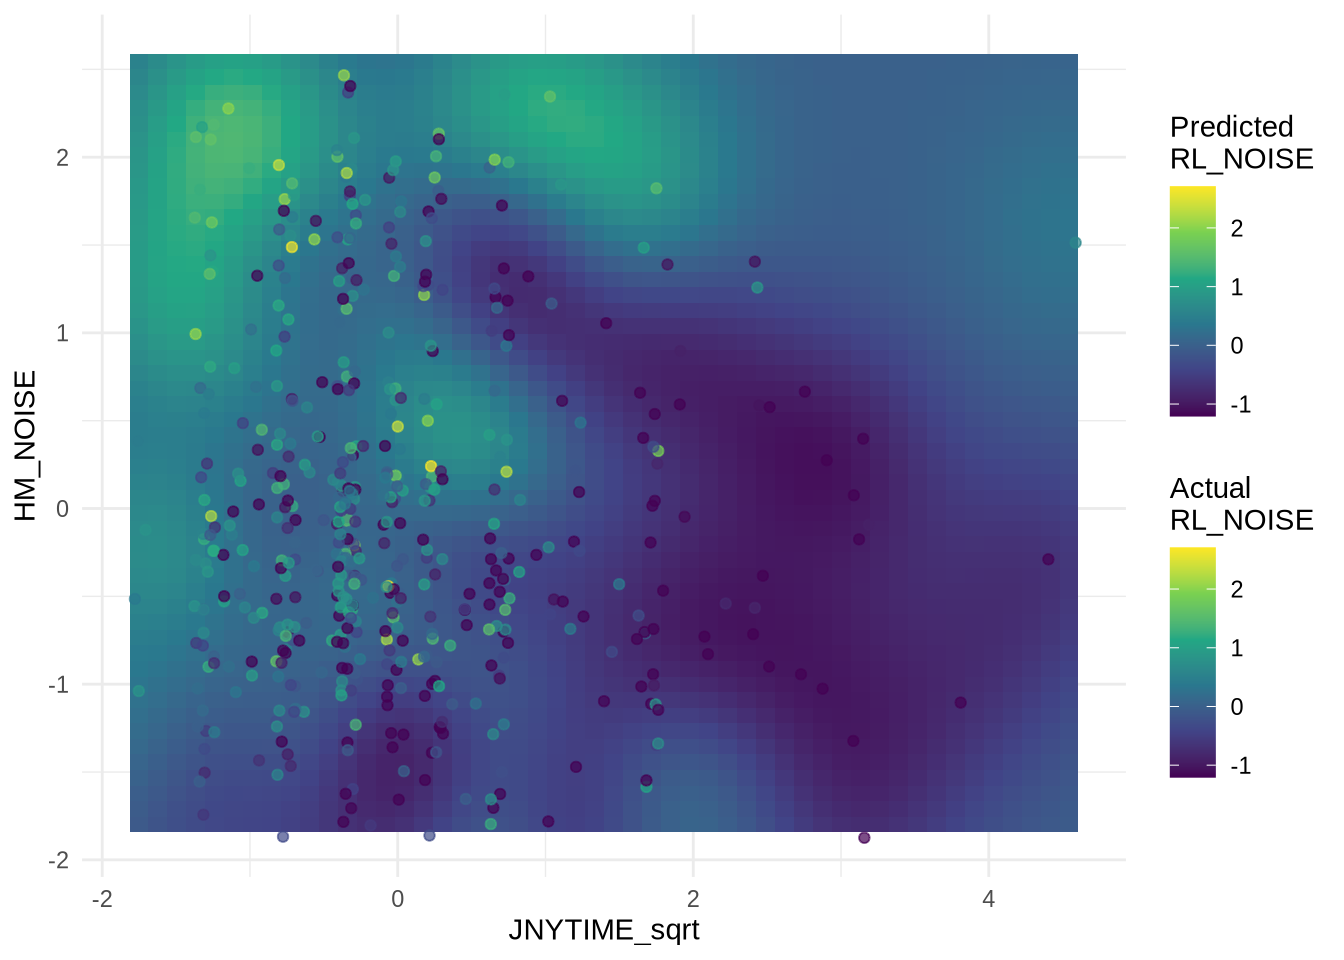
\includegraphics[keepaspectratio]{index_files/figure-latex/notebooks-RL-via-HM-fig-predicted-rl-noise-w-gp-output-1.png}}

}

\caption{\label{fig-predicted-rl-noise-w-gp}}

\end{figure}%

\textsubscript{Source:
\href{https://LGraz.github.io/wsl--prs-analysis/notebooks/RL-via-HM-preview.html\#cell-fig-predicted-rl-noise-w-gp}{Predict
RL via HM}}

\subsubsection{Soundscape Description per
HM\_Noise}\label{soundscape-description-per-hm_noise}

\begin{figure}[H]

\centering{

\pandocbounded{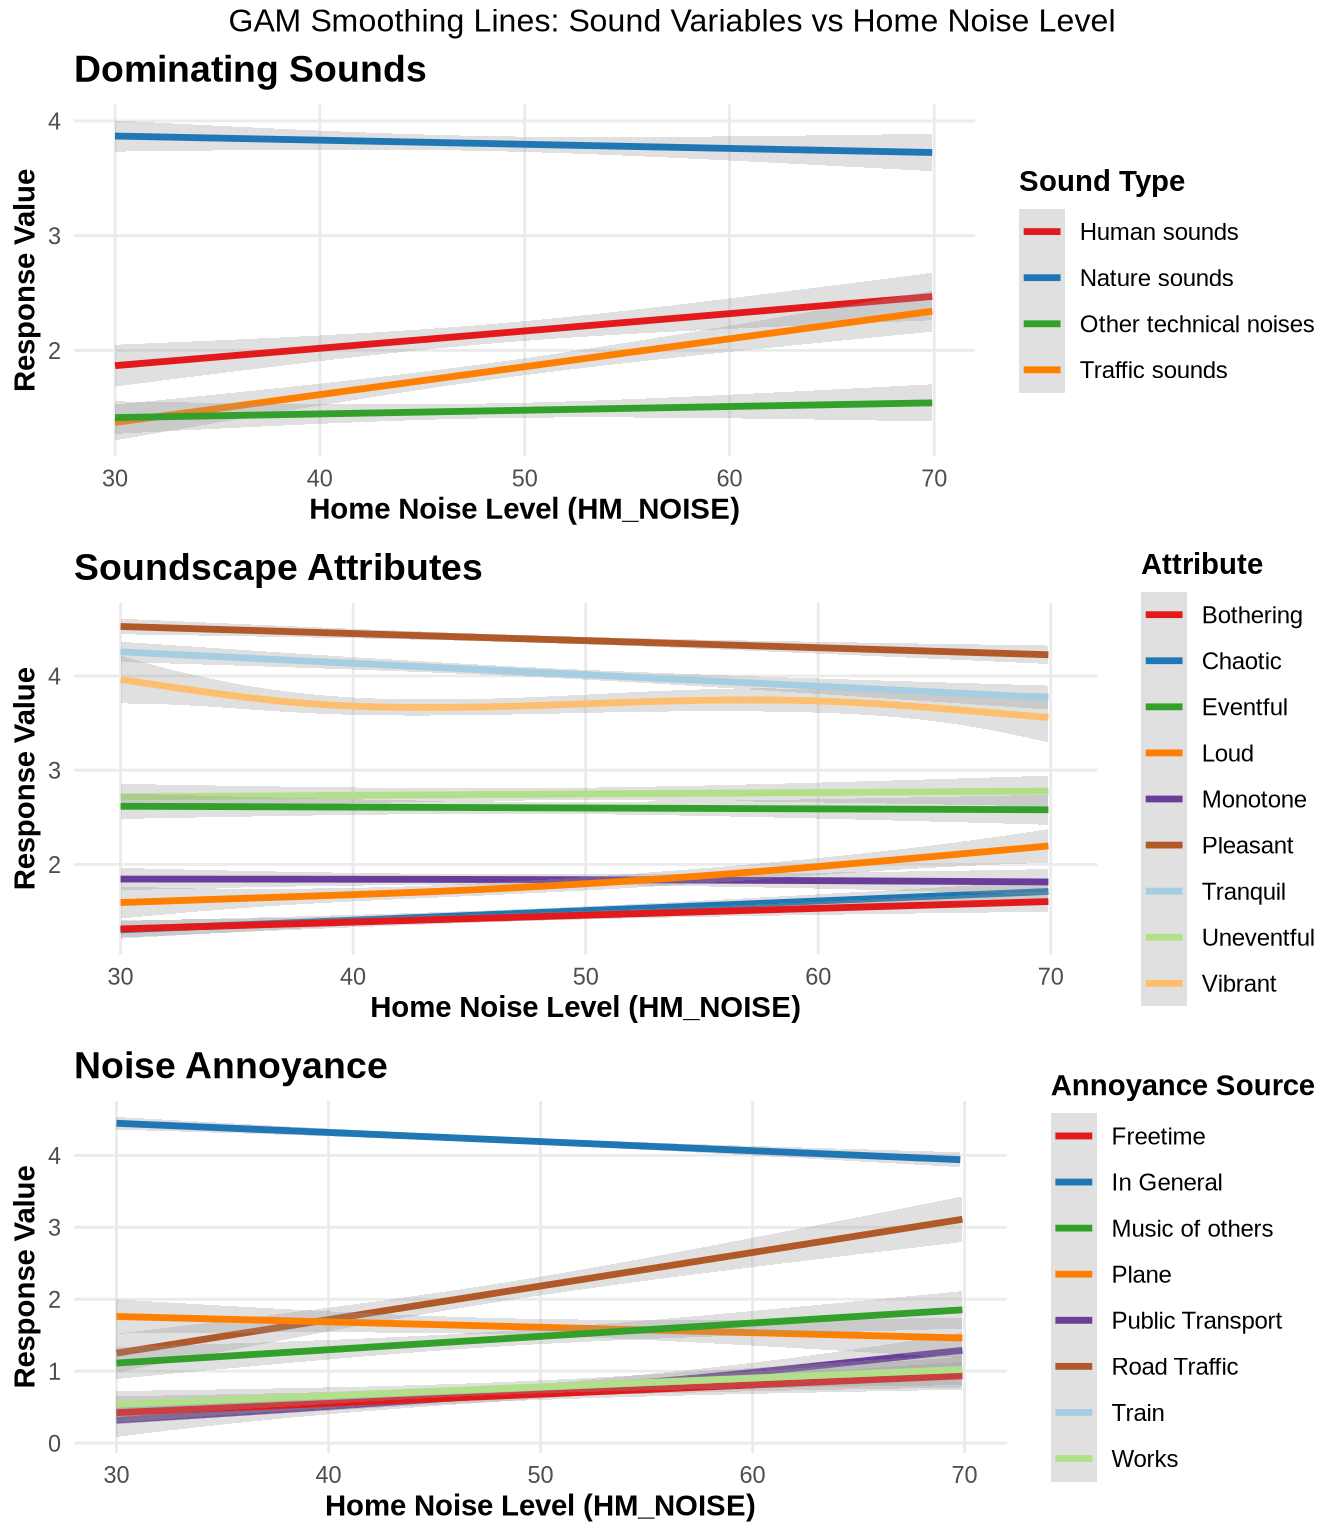
\includegraphics[keepaspectratio]{index_files/figure-latex/notebooks-RL-via-HM-fig-soundscape-description-output-1.png}}

}

\caption{\label{fig-soundscape-description}}

\end{figure}%

\textsubscript{Source:
\href{https://LGraz.github.io/wsl--prs-analysis/notebooks/RL-via-HM-preview.html\#cell-fig-soundscape-description}{Predict
RL via HM}}




\end{document}
